\section{Op Amp 741}

\subsection{Pengantar Op Amp 741}

\begin{frame}{Pengantar Op Amp 741}
	\begin{itemize}
		\item Monolitic amp $ \mu\text{A709} $ dibuat tahun 1965 oleh Fairchild Semiconductor
		\item Meskipun tergolong sukses, generasi pertama op amp ini memiliki kekurangan maka dibuatlah $ \mu\text{A741} $
		\item Karena harganya yang tidak mahal dan mudah digunakan, $ \mu\text{A741} $ sangatlah sukses.
		\item Banyak manufaktur yang membuat $ \mu\text{A741} $:
		\begin{itemize}
			\item ON Semiconductor: MC1741
			\item Texas Instruments: LM741
			\item Analog Devices: AD741.
		\end{itemize}
		\item Istilah umumnya op amp 741
	\end{itemize}
\end{frame}

\subsection{Standar Industri}

\begin{frame}{Standar Industri}
	\begin{itemize}
		\item Tipe 741 memiliki beberapa versi: 741, 741A, 741C, 741E, dan 741N
		\item Bergantung pada karakteristiknya (voltage gain, temp. range, noise level, dll)
		\item 741C (C = \textit{Commercial grade}) $ \rightarrow $ sedikit lebih murah dan paling banyak digunakan
		\item $ A_{VOL} = 100000 $, $ z_{in} = 2 \text{ M}\Omega $, $ z_out = 75~\Omega $
		\item Gambar \ref{fig-16.03} menunjukkan 3 package yang terkenal beserta pinoutnya
	\end{itemize}
\end{frame}

\begin{frame}{Standar Industri}
	\begin{figure}
		\centering
		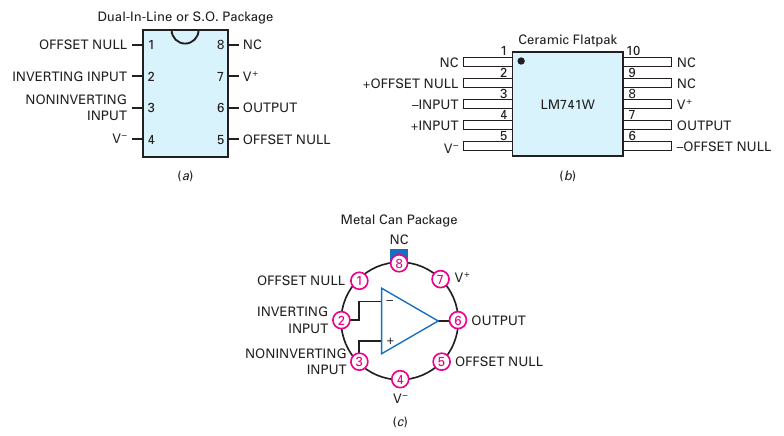
\includegraphics[width=0.7\linewidth]{gambar/fig-16.03}
		\caption{Op amp 741 pinouts (a) dual-in-line, (b) ceramic flatpak, (c) metal can}
		\label{fig-16.03}
	\end{figure}
\end{frame}

\subsection{Diagram skematik yang disederhanakan dari 741}

\begin{frame}{Diagram skematik yang disederhanakan dari 741}
	\begin{figure}
		\centering
		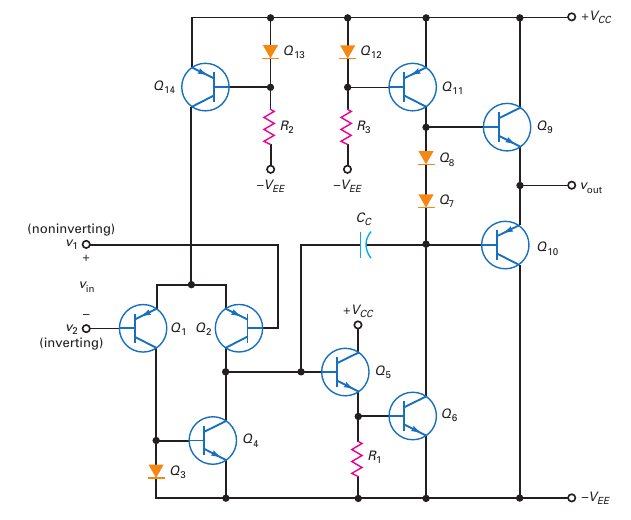
\includegraphics[height=0.7\textheight]{gambar/fig-16.04}
		\caption{Rangkaian ekivalen dari op amp 741}
		\label{fig-16.04}
	\end{figure}
\end{frame}

\subsection{Input Diff Amp}

\begin{frame}{Input Diff Amp}
	\begin{itemize}
		\item Gambar \ref{fig-16.04} adalah diagram skematik yang disederhanakan dari 741.
		\item Rangkaian ini merupakan ekivalen dari 741 dan op amp generasi-generasi selanjutnya.
		\item Tidak perlu memahami secara detail rangkaian tersebut, cukup pahami ide dasarnya saja.
	\end{itemize}
\end{frame}

\begin{frame}{Input Diff Amp}
	\begin{itemize}
		\item Input stage yang digunakan adalah diff amp ($ Q_1 $ dan $ Q_2 $).
		\item $ Q_{14} $ adalah sumber arus yang menggantikan tail resistor.
		\item $ R_2 $, $ Q_{13} $, $ Q_{14} $ adalah current mirror yang menghasilkan tail current untuk $ Q_1 $ dan $ Q_2 $.
		\item Daripada menggunakan resistor biasa sebagai resistor kolektor, 741 ini menggunakan active-load resistor.
		\item Active-load $ Q_4 $ bertindak sebagai seperti sumber arus dengan impedansi yang sangat tinggi.
		\item Akibatnya, voltage gain dari diff amp menjadi jauh lebih besar daripada menggunakan passive-load resistor.
	\end{itemize}
\end{frame}

\begin{frame}{Input Diff Amp}
	\begin{itemize}
		\item Sinyal yang dikuatkan dari diff amp akan mendrive base dari $ Q_5 $, sebuah emitter follower.
		\item Stage ini akan menaikkan level impedansi untuk menghindari loading down dari diff amp.
		\item Sinyal yang keluar dari $ Q_5 $ menuju ke $ Q_6 $.
		\item Dioda $ Q_7 $ dan $ Q_8 $ adalah bagian dari bias untuk final stage.
		\item $ Q_{11} $ adalah active-load resistor untuk $ Q_6 $, sehingga $ Q_6 $ dan $ Q_{11} $ seperti CE driver stage dengan voltage gain yang sangat besar.
		\item Simbol dioda digunakan ketika transistor memiliki base yang terhubung singkat dengan collector, seperti $ Q_3 $.
	\end{itemize}
\end{frame}

\subsection{Final Stage}

\begin{frame}{Final Stage}
	\begin{itemize}
		\item Sinyal yang dikuatkan yang keluar dari CE driver stage ($ Q_6 $) menuju ke final stage, yang merupakan Class-B push-pull emitter follower ($ Q_9 $ dan $ Q_{10} $).
		\item Karena supply tegangan yang terbagi menjadi 2 (Positif $ V_CC $ dan negatif $ V_EE $), quiescent output idealnya adalah 0 V ketika tegangan inputnya nol.
		\item Deviasi berapapun dari 0 V disebut tegangan error output (output error voltage).
		\item Jika $ v_1 > v_2 $, tegangan input $ v_{in} $ akan menghasilkan tegangan output $ v_{out} $ positif. Sebaliknya, jika $ v_2 > v_1 $, tegangan input $ v_{in} $ akan menghasilkan tegangan output $ v_{out} $ negatif.
		\item Idealnya , $ v_{out} $ bisa sama positifnya dengan $ +V_{CC} $ dan sama negatifnya dengan $ -V_{EE} $ sebelum clipping terjadi.
		\item Output swing normalnya dalam 1 hingga 2 V dari tiap tegangan supply karena tegangan drop di dalam 741.
	\end{itemize}
\end{frame}

\subsection{Active Loading}

\begin{frame}{Active Loading}
	\begin{itemize}
		\item Pada Gambar \ref{fig-16.04}, terdapat 2 active-loading (menggunakan transistor daripada resistor sebagai load atau bebannya).
		\item Pertama, ada active-load $ Q_4 $ di input diff.
		\item Kedua, ada active-load $ Q_{11} $ do CE driver stage.
		\item Karena sumber arus memiliki impedansi output yang besar, active-load menghasilkan voltage gain yang lebih besar daripada jika menggunakan resistor.
		\item Active-load ini umumnya menghasilkan voltage gain sebesar 100000 untuk 741C.
		\item Active-load sangat populer di dalam IC karena lebih mudah dan lebih murah untuk membuat transistor di dalam chip daripada membuat resistor.
	\end{itemize}
\end{frame}

\subsection{Frequency Compensation}

\begin{frame}{Frequency Compensation}
	\begin{itemize}
		\item Pada Gambar \ref{fig-16.04}, $ C_c $ adalah compensating capacitor.
		\item Karena efek Miller, kapasitor kecil ini (umumnya 30 pF) dikalikan dengan voltage gain dari $ Q_5 $ dan $ Q_6 $ untuk mendapatkan kapasitansi ekivalen yang lebih besar yaitu\\
		$$ C_{in(M)} = (A_v + 1) C_c $$ \\
		di mana $ A_v $ adalah voltage gain dari stage $ Q_5 $ dan $ Q_6 $.
		\item Resistansi yang berhadapan dengan kapasitansi Miller adalah impedansi output dari diff amp sehingga kita memiliki rangkaian lag.
		\item Rangkaian lag menghasilkan cut off frequency 10 Hz di 741C.
		\item Open-loop gain dari op amp adalah di bawah 3 dB di cut off frequency ini.
		\item Kemudian, $ A_{VOL} $ menurun sekitar 20 dB/decade hingga mencapai unity-gain frequency.
	\end{itemize}
\end{frame}

\begin{frame}{Frequency Compensation}
	\begin{figure}
		\centering
		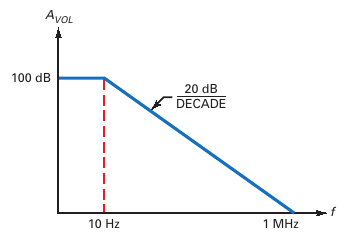
\includegraphics[width=0.5\linewidth]{gambar/fig-16.05}
		\caption{Bode plot $ A_{VOL} $ 741C ideal}
		\label{fig-16.05}
	\end{figure}
\end{frame}

\begin{frame}{Frequency Compensation}
	\begin{itemize}
		\item Gambar \ref{fig-16.05} menunjukkan Bode plot ideal dari open-loop voltage gain terhadap frequency.
		\item 741C memiliki open-loop voltage gain sebesar 100000, ekivalen dengan 100 dB.
		\item Karena open-loop cut off frequency adalah 10 Hz, voltage gain akan berhenti di 10 Hz dan turun sebesar 20 dB/decade hingga 0 dB di 1 MHz.
	\end{itemize}
\end{frame}

\subsection{Bias \& Offset}

\begin{frame}{Bias \& Offset}
	\begin{itemize}
		\item Telah dijelaskan sebelumnya bahwa diff amp memiliki input bias dan offset yang menghasikan error output ketika tidak ada input sinyal.
		\item Dalam beberapa aplikasi, output error adalah cukup kecil untuk diabaikan.
		\item Tapi ketika output error tidak bisa diabaikan, designer dapat mereduksinya dengan menggunakan base resistor yang bernilai sama.
		\item Cara ini dapat menghilangkan permasalahan dari arus bias tapi tidak unutk arus offset dan tegangan offset.	
	\end{itemize}
\end{frame}

\begin{frame}{Bias \& Offset}
	\begin{itemize}
		\item Sehingga cara terbaik untuk menghilangkan error output adalah dengan menggunakan nulling circuit yang diberikan di datasheet.
		\item Nulling circuit dapat menghilangkan output error dan meminimalkan thermal drift, perubahan yang pelan di tegangan output yang disebabkan oleh perubahan temperatur pada parameter op amp.
		\item Terkadang datasheet tidak menyertakan nulling circuit, sehingga kita berikan tegangan input yang kecil untuk me-null-kan output.
	\end{itemize}
\end{frame}

\begin{frame}{Bias \& Offset}
	\begin{figure}
		\centering
		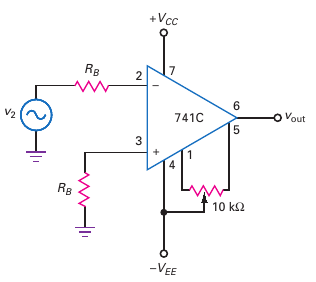
\includegraphics[height=0.7\textheight]{gambar/fig-16.06}
		\caption{Penggunaan compensation dan nulling 741C}
		\label{fig-16.06}
	\end{figure}
\end{frame}

\begin{frame}{Bias \& Offset}
	\begin{itemize}
		\item Gambar \ref{fig-16.06} menunjukkan metode nulling yang disarankan oleh datasheet 741C.
		\item Sumber AC men-drive inverting input yang memiliki resistansi Thevenin $ R_B $.
		\item Untuk menetralkan efek dari arus bias input (80 nA) yang mengalir melalui resistor ini, resistor diskret yang bernilai sama ditambahkan ke noninverting input seperti di gambar tersebut.
	\end{itemize}
\end{frame}

\begin{frame}{Bias \& Offset}
	\begin{itemize}
		\item Untuk menghilangkan efek dari arus offset input 20 nA dan tegangan offset input 2 mV, datasheet 741C merekomendasikan untuk menggunakan 10 k$ \Omega $ potentiometer antara pon 1 dan pin 5.
		\item Dengan meng-adjust potensiometer ini dengan tanpa sinyal input, kita dapat membuat tegangan output menjadi nol.
	\end{itemize}
\end{frame}

\subsection{CMRR, MPP, dan $A_{VOL}$}

\begin{frame}{CMRR, MPP, dan $A_{VOL}$}
	\begin{figure}
		\centering
		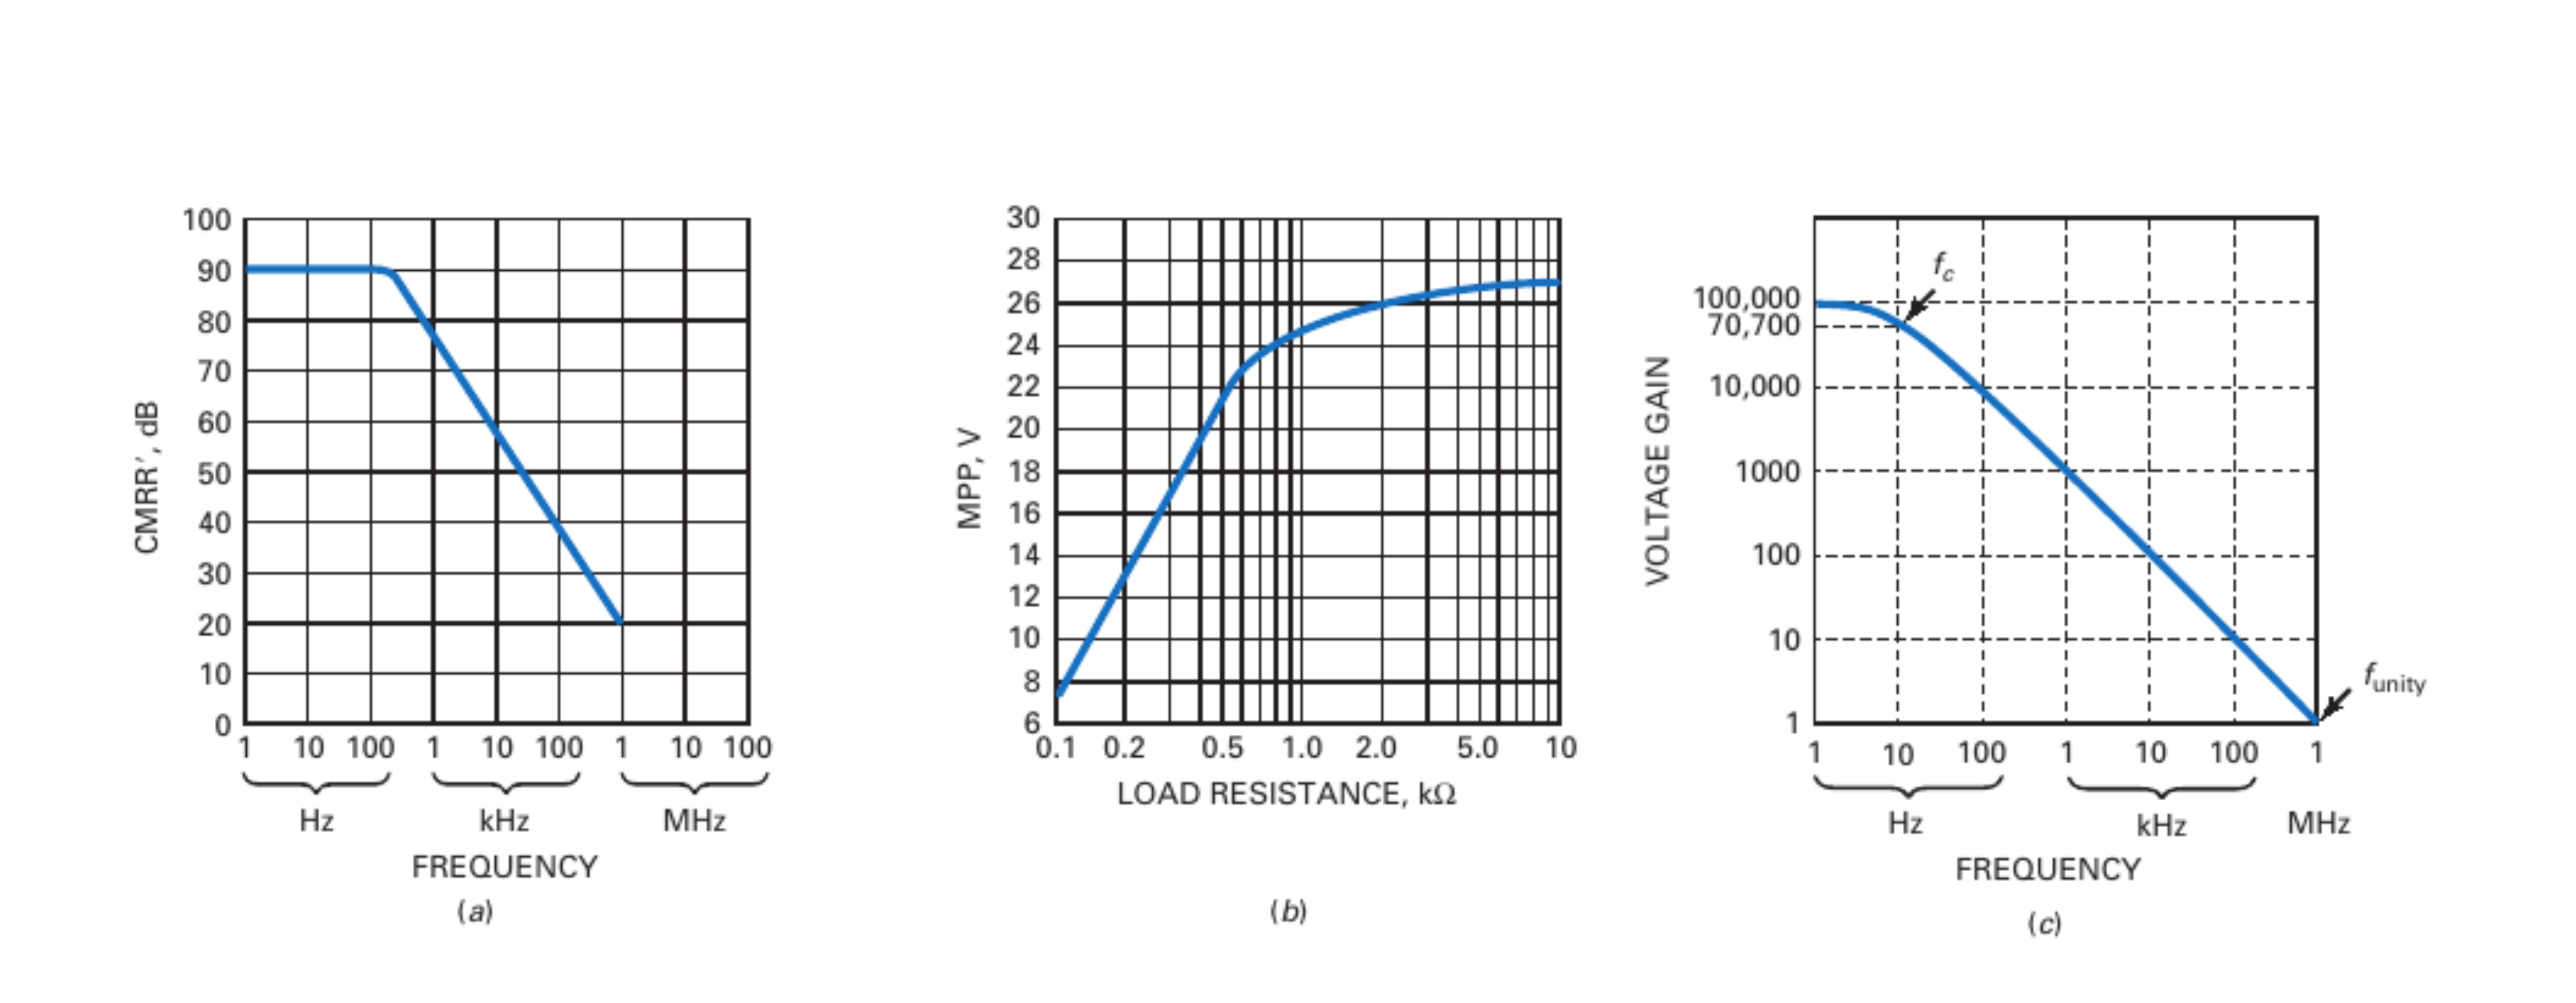
\includegraphics[width=\linewidth]{gambar/fig-16.07}
		\caption{Grafik (a) Common-Mode Rejection Ratio (CMRR), (b) Maximum Peak-to-Peak Output (MPP), dan (c) Open-Loop Voltage Gain $A_{VOL}$ dari 741C}
		\label{fig-16.07}
	\end{figure}
\end{frame}

\subsection{Common-Mode Rejection Ratio}

\begin{frame}{Common-Mode Rejection Ratio}
	\begin{itemize}
		\item Untuk 741C, CMRRnya adalah 90 dB di frekuensi rendah.
		\item Jika diberikan 2 sinyal yang sama, sinyal yang diinginkan dan yang tidak, sinyal yang diinginkan akan bernilai 90 dB lebih besar di output daripada common-mode signal-nya.
		\item Atau sinyal yang diinginkan 30000 kali lebih besar daripada common-mode signal.
		\item Pada frekuensi tinggi, efek reaktif menurunkan CMRR seperti yang ditunjukkan oleh Gambar \ref{fig-16.07}a.
	\end{itemize}
\end{frame}

\subsection{Maximum Peak-to-Peak Output}

\begin{frame}{Maximum Peak-to-Peak Output}
	\begin{itemize}
		\item Nilai MPP dari amplifier adalah output peak-to-peak maksimum yang amplifier dapat hasilkan tanpa clipping.
		\item Karena quiescent output dari op amp idealnya bernilai nol, tegangan output ac dapat berayun secara positif atau negatif.
		\item Untuk resistansi beban yang lebih besar daripada $ R_{out} $, tegangan output dapat berayun hampir ke tegangan supply.
		\item Contoh, jika $ V_{CC} $ = +15 V dan $ V_{EE} $ = - 15 V, nilai MPP dengan resistansi beban sebesar 10 k$ \Omega $ idealnya adalah 30 V.
	\end{itemize}
\end{frame}

\begin{frame}{Maximum Peak-to-Peak Output}
	\begin{itemize}
		\item Dengan op amp yang tidak ideal, output tidak dapat berayun ke tegangan supply karena ada tegangan drop yang kecil di final stage op amp.
		\item Ketika resistansi beban tidak besar dibandingkan dengan $ R_{out} $, beberapa tegangan yang dikuatkan akan drop di $ R_{out} $, artinya tegangan output final lebih kecil.
		\item Gambar \ref{fig-16.07}b menunjukkan MPP vs resistansi beban untuk 741C dengan tegangan supply +15 V dan -15 V
		\item Perhatikan bahwa MPP sekitar 27 V untuk $ R_L $ 10 k$ \Omega $.
		\item Artinya, output saturasi secara positif +13.5 V dan secara negatif -13.5 V.
		\item Ketika resistansi beban menurun, MPP juga menurun.
		\item Contohnya, jika resistansi beban 275 $\Omega$, MPP menurun hingga 16 V, yang artinya output saturasi secara positif +8 V dan secara negatif -8 V.
	\end{itemize}
\end{frame}

\subsection{Short-Circuit Current}

\begin{frame}{Short-Circuit Current}
	\begin{itemize}
		\item Di beberapa aplikasi, op amp mungkin men-drive resistansi beban sekitar nol.
		\item Pada kasus seperti ini, kita perlu mengetahui nilai dari short-circuit output current.
		\item Datasheet dari 741C menyatakan short-circuit output current sebesar 25 mA.
		\item Ini adalah arus output maksimum yang op amp hasilkan.
		\item Jika kita menggunakan resistor beban yang lebih kecil (kurang dari 75 $\Omega$), jangan harap untuk mendapatkan tegangan output yang besar karena tegangannya tidak akan lebih besar daripada 25 mA dikali dengan resistansi beban tadi.
	\end{itemize}
\end{frame}

\subsection{Frequency Response}

\begin{frame}{Frequency Response}
	\begin{itemize}
		\item Gambar \ref{fig-16.07}c menunjukkan respon frekuensi dari sinyal yang kecil dari 741C.
		\item Pada frekuensi tengah, voltage gain sebesar 100000.
		741C memiliki cutoff frequency $ f_c $ di 10 Hz.
		\item Seperti yang ditampilkan, voltage gain sebesar 70700 (menurun 3 dB) di 10 Hz.
		\item Di atas cutoff frequency, voltage gain akan menurun sebesar 20 dB/decade.
	\end{itemize}
\end{frame}

\begin{frame}{Frequency Response}
	\begin{itemize}
		\item Unity-gain frequency adalah frekuensi dimana voltage gain bernilai 1.
		\item Pada Gambar \ref{fig-16.07}c, $ f_{unity} $ adalah 1 MHz.
		\item Datasheet biasanya menspesifikkan nilai dari $ f_{unity} $ karena ini merepresentasikan batas atas pada gain yang dapat digunakan di op amp.
		\item Contoh, datasheet 741C menyatakan $ f_{unity} $ sebesar 1 MHz. Artinya 741C dapat menguatkan sinyal hingga 1 MHz.
		\item Di atas 1 MHz, voltage gain kurang dari 1 dan 741C tidak berguna.
		\item Jika menginginkan $ f_{unity} $ yang lebih tinggi, gunakan LM318 yang memiliki $ f_{unity} $ 15 Hz.
	\end{itemize}
\end{frame}

\subsection{Slew Rate}

\begin{frame}{Slew Rate}
	\begin{itemize}
		\item Compensating capacitor di dalam 741C memberikan fungsi yang sangat penting.
		\item Yaitu mencegah osilasi yang dapat menginterferensi sinyal yang diinginkan.
		\item Namun ada kekurangan, compensating capacitor perlu di-charge dan di-discharge.
		\item Hal ini membuat batasan pada seberapa cepat output op amp dapat berubah.
	\end{itemize}
\end{frame}

\begin{frame}{Slew Rate}
	\begin{itemize}
		\item Tegangan input ke op amp adalah tegangan step positif, transisi tegangan yang mendadak dari satu level dc ke level dc yang lebih tinggi.
		\item Jika op amp nya sempurna, maka kita memperoleh respons ideal seperti pada Gambar \ref{fig-16.08}a.
		\item Namun, output yang terjadi adalah sinyal eksponensial positif.
		\item Hal ini terjadi karena compensating capacitor harus di-charge terlebih dahulu sebelum tegangan output dapat berubah ke level yang lebih tinggi.
	\end{itemize}
\end{frame}

\begin{frame}{Slew Rate}
	\begin{figure}
		\centering
		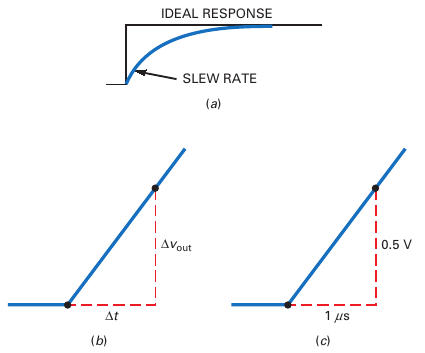
\includegraphics[height=0.7\textheight]{gambar/fig-16.08}
		\caption{(a) Respon ideal dan aktual terhadap tegangan step input, (b) ilustrasi definisi slew rate, (c) $ S_R = 0.5 \text{ V/}\mu\text{s} $}
		\label{fig-16.08}
	\end{figure}
\end{frame}

\begin{frame}{Slew Rate}
	\begin{itemize}
		\item Initial slope dari bentuk sinyal eksponensial disebut slew rate, $ S_R $.
		\item Persamaan slew rate, $ S_R $.
		\begin{equation}\label{pers.16.1}
			S_R = \frac{\Delta v_{out}}{\Delta t}
		\end{equation}
		\item Gambar \ref{fig-16.08}b mengilustrasikan makna dari slew rate.
		\item Initial slope = perubahan vertikal dibagi dengan perubahan hoorizontal di antara 2 titik di bagian awal gelombang eksponensial.
		\item Exponential wave meningkat 0.5 V selama 1 mikrodetik pertama, maka
		\begin{align*}
			S_R &= \frac{\Delta v_{out}}{\Delta t} = \frac{0.5 \text{ V}}{1~\mu\text{s}} \\
			&= 0.5 \text{ V/}\mu\text{s}
		\end{align*}
	\end{itemize}
\end{frame}

\begin{frame}{Slew Rate}
	\begin{itemize}
		\item Slew rate merepresentasikan respon tercepat yang dimiliki oleh op amp.
		\item Contoh, slew rate dari 741C adalah 0.5 V/$\mu$s.
		\item Artinya adalah output dari 741C dapat berubah tidak lebih cepat dari 0.5 V dalam 1 mikrodetik.
		\item Dengan kata lain, jika 741C di-drive oleh tegangan inpun step, maka kita tidak mendapatkan tegangan output step tapi kita mendapatkan gelombang output exponensial.
	\end{itemize}
\end{frame}

\begin{frame}{Slew Rate}
	\begin{itemize}
		\item Slew rate dapat dibatasi dengan sinyal sinusoidal.
		\item Gambar \ref{fig-16.09}a, op amp dapat menghasilkan gelombang sinus output hanya jika initial slope dari gelombang sinus kurang dari slew rate.
		\item Contoh, jika gelombang sinus output memiliki initial slope 0.1 V/$\mu$s, 741C dapat menghasilkan gelombang sinus tanpa masalah sama sekali karena slew rate 741C adalah 0.5 V/$\mu$s.
		\item Di lain sisi, jika gelombang sinus memiliki initial slope 0.1 V/$\mu$s, output lebih kecil dari pada initial slope gelombang sinus maka output akan terlihat triangular daripada sinusoidal seperti yang ditambilkan pada Gambar \ref{fig-16.09}b.
	\end{itemize}
\end{frame}

\begin{frame}{Slew Rate}
	\begin{figure}
		\centering
		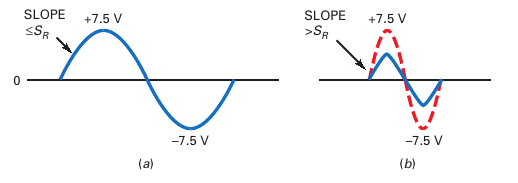
\includegraphics[width=0.7\linewidth]{gambar/fig-16.09}
		\caption{(a) Initial slope dari gelombang sinus, (b) distorsi terjadi jika initial slope melebihi slew rate}
		\label{fig-16.09}
	\end{figure}
\end{frame}

\begin{frame}{Slew Rate}
	\begin{itemize}
		\item Datasheet op amp selalu menentukan slew rate karena nilai ini membatasi respon sinyal yang besar dari op amp.
		\item Jika gelombang sinus output sangat kecil atau frekuensinya sangat kecil maka slew rate bukan masalah.
		\item Namun jika sinyal output besar dan frekuensinya sangat besar maka slew rate akan mendistorsi sinyal output
	\end{itemize}
\end{frame}

\begin{frame}{Slew Rate}
	\begin{itemize}
		\item Kita akan turunkan persamaan berikut ini:
		\[ S_S = 2 \pi f V_p \]
		\item $ S_s $: initial slope dari gelombang sinus, $ f $: frekuensi, $ V_p $: nilai peak.
		\item Untuk menghindari slew-rate distortion dari gelombang sinus, $ S_S $ harus lebih kecil atau sama dengan $ S_R $, maka
		\begin{align*}
			S_S &\leq S_R \\
			2 \pi f V_p &\leq S_R \\
			f &\leq \frac{S_R}{2 \pi V_p} \\
		\end{align*}
	\end{itemize}
\end{frame}

\begin{frame}{Slew Rate}
	\begin{itemize}
		\item Sehingga
			\begin{equation} \label{pers.16.2}
				f_{max} = \frac{S_R}{2 \pi V_p}
			\end{equation}
		\item $ f_{max} $ adalah frekuensi tertinggi yang dapat dikuatkan tanpa slew-rate distortion.
		\item $ f_{max} $ disebut juga power bandwidth.
		\item Gambar \ref{fig-16.10} menunjukkan grafik dari tiga slew rate. $ S_R $ = 0.5 V/$\mu$S untuk 741C dan 
	\end{itemize}
\end{frame}


\begin{frame}{Slew Rate}
	\begin{figure}
		\centering
		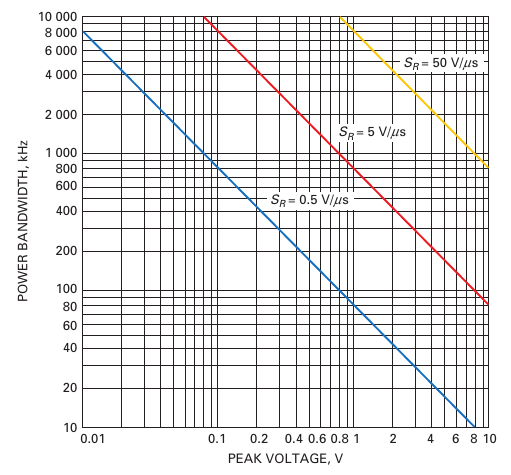
\includegraphics[height=0.7\textheight]{gambar/fig-16.10}
		\caption{Grafik power bandwidth vs. peak voltage}
		\label{fig-16.10}
	\end{figure}
\end{frame}

\begin{frame}{Slew Rate}
	\begin{itemize}
		\item Misalkan kita menggunakan 741C.
		\item Agar kita bisa mendapatkan tegangan peaak output sebesar 8 V tanpa distorsi, frekuensi tidak boleh lebih besar daripada 10 kHz.
		\item Untuk meningkatkan $ f_{max} $, kecilkan tegangan output.
		\item Misalkan, tegangan peak output 1 V maka $ f_{max} $ meningkat menjadi 80 kHz.
	\end{itemize}
\end{frame}

\subsection{Contoh Soal 2.1}
\begin{frame}{Contoh Soal 2.1}
	\begin{multicols}{2}
		\begin{center}
			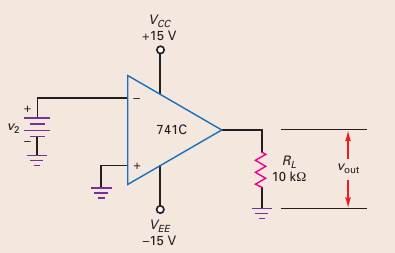
\includegraphics[width=\linewidth]{gambar/fig-16.11a}
		\end{center}
		\columnbreak
		\begin{itemize}
			\item Pertanyaan:
			\begin{itemize}
				\item Berapa tegangan inverting input yang dibutuhkan untuk men-drive op amp 741C hingga saturasi negatif?
			\end{itemize}
		\end{itemize}
	\end{multicols}
\end{frame}

\begin{frame}{Contoh Soal 2.1}
	\begin{multicols}{2}
		\begin{center}
			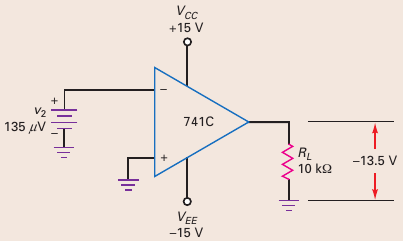
\includegraphics[width=\linewidth]{gambar/fig-16.11b}
		\end{center}
		\columnbreak
		\begin{itemize}
			\item Jawaban:
			\begin{itemize}
				\item Berdasarkan Gambar \ref{fig-16.07} (b), $ \text{MPP} = 27 \text{ V} $ untuk $ R_L = \text{ k}\Omega $
				\item Sehingga tegangan output negatif saturasinya = - 13.5 V
				\item Karena $ A_{VOL} = 100000 $, maka tegangan input yang dibutuhkan:
				\begin{align*}
					v_2 &= \frac{v_{out}}{A_{VOL}} \\
					&= \frac{13.5 \text{ V}}{100000} = 135 ~\mu\text{V}
				\end{align*}
			\end{itemize}
		\end{itemize}
	\end{multicols}
\end{frame}

\subsection{Latihan Soal 2.1}
\begin{frame}{Latihan Soal 2.1}
	\begin{multicols}{2}
		\begin{center}
			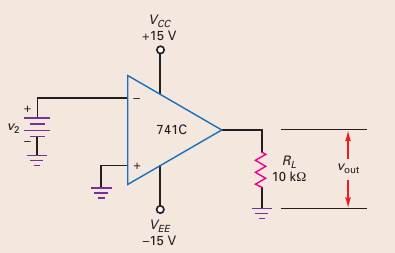
\includegraphics[width=\linewidth]{gambar/fig-16.11a}
		\end{center}
		\columnbreak
		\begin{itemize}
			\item Pertanyaan:
			\begin{itemize}
				\item Berapa tegangan inverting input yang dibutuhkan untuk men-drive op amp 741C hingga saturasi negatif jika $ A_{VOL} = 200000 $ ?
			\end{itemize}
		\end{itemize}
	\end{multicols}
\end{frame}

\subsection{Contoh Soal 2.2}
\begin{frame}{Contoh Soal 2.2}
	\begin{itemize}
		\item Pertanyaan:
		\begin{itemize}
			\item Berapa common-mode rejection ratio (CMRR) dari 741C ketika frekuensi input-nya adalah 100 kHz?
		\end{itemize}
		\item Jawaban:
		\begin{itemize}
			\item Berdasarkan Gambar \ref{fig-16.07} (a), $ \text{CMRR}_{\text{dB}} \approx 40 \text{ dB} $ di 100 kHz.
			\[ \text{CMRR} = 10^{(\text{CMRR}_{\text{dB}}/20)} = 10^{(40 \text{ dB}/20)} = 100\]
		\end{itemize}
	\end{itemize}
\end{frame}

\subsection{Latihan Soal 2.2}
\begin{frame}{Latihan Soal 2.2}
	\begin{itemize}
		\item Pertanyaan:
		\begin{itemize}
			\item Berapa common-mode rejection ratio (CMRR) dari 741C ketika frekuensi input-nya adalah 10 kHz?
		\end{itemize}
	\end{itemize}
\end{frame}

\subsection{Contoh Soal 2.3}
\begin{frame}{Contoh Soal 2.3}
	\begin{itemize}
		\item Pertanyaan:
		\begin{itemize}
			\item Berapa open-loop voltage gain dari 741C jika frekuensi input-nya adalah 1 kHz ? 10 kHz ? 100 kHz ?
		\end{itemize}
		\item Jawaban:
		\begin{itemize}
			\item Berdasarkan Gambar \ref{fig-16.07} (c), voltage gain-nya adalah 1000 untuk 1 kHz, 100 untuk 10 kHz, dan 10 untuk 100 kHz.
		\end{itemize}
	\end{itemize}
\end{frame}

\subsection{Contoh Soal 2.4}
\begin{frame}{Contoh Soal 2.4}
	\begin{itemize}
		\item Pertanyaan:
		\begin{itemize}
			\item Tegangan input ke op amp adalah tegangan fungsi step. Output-nya adalah sebuah waveform eksponensial yang berubah ke 0.25 V dalam 0.1 $ \mu \text{s} $. Berapa slew rate dari op amp tersebut?
		\end{itemize}
		\item Jawaban:
		\begin{itemize}
			\item Berdasarkan Persamaan \ref{pers.16.1}
			\[ S_R = \frac{\Delta v_{out}}{\Delta t} = \frac{0.25 \text{ V}}{0.1 ~\mu \text{s}} = 2.5 \text{ V/}\mu \text{s}\]
		\end{itemize}
	\end{itemize}
\end{frame}

\subsection{Latihan Soal 2.4}
\begin{frame}{Latihan Soal 2.4}
	\begin{itemize}
		\item Pertanyaan:
		\begin{itemize}
			\item Tegangan input ke op amp adalah tegangan fungsi step. Output-nya adalah sebuah waveform eksponensial yang berubah ke 0.8 V dalam 0.2 $ \mu \text{s} $. Berapa slew rate dari op amp tersebut?
		\end{itemize}
	\end{itemize}
\end{frame}

\subsection{Contoh Soal 2.5}
\begin{frame}{Contoh Soal 2.5}
	\begin{itemize}
		\item Pertanyaan:
		\begin{itemize}
			\item Op amp LF411A dengan slew rate $ 	15 \text{ V/}\mu \text{s} $. Berapa power bandwidth dari tegangan peak output 10 V ?
		\end{itemize}
		\item Jawaban:
		\begin{itemize}
			\item Berdasarkan Persamaan \ref{pers.16.2}
			\[ f_{max} = \frac{S_R}{2 \pi V_p} = \frac{15 \text{ V/}\mu \text{s}}{2 \pi (10 \text{ V}) } = 239 \text{ kHz}\] 
		\end{itemize}
	\end{itemize}
\end{frame}

\subsection{Latihan Soal 2.5}
\begin{frame}{Latihan Soal 2.5}
	\begin{itemize}
		\item Pertanyaan:
		\begin{itemize}
			\item Op amp LF411A dengan slew rate $ 	15 \text{ V/}\mu \text{s} $. Berapa power bandwidth dari tegangan peak output 200 mV ?
		\end{itemize}
	\end{itemize}
\end{frame}

\subsection{Contoh Soal 2.6}
\begin{frame}{Contoh Soal 2.6}
	\begin{itemize}
		\item Pertanyaan:
		\begin{itemize}
			\item Berapa power bandwidth dari:
			\begin{itemize}
				\item $ S_R = 0.5 \text{ V/}\mu\text{s} $ dan $ V_p = 8 \text{ V} $ 
				\item $ S_R = 5 \text{ V/}\mu\text{s} $ dan $ V_p = 8 \text{ V} $ 
				\item $ S_R = 50 \text{ V/}\mu\text{s} $ dan $ V_p = 8 \text{ V} $ 
			\end{itemize}
		\end{itemize}
		\item Jawaban:
		\begin{itemize}
			\item Berdasarkan Gambar \ref{fig-16.10}
			\begin{itemize}
				\item $ f_{max} = 10 \text{ kHz}$ 
				\item $ f_{max} = 100 \text{ kHz}$
				\item $ f_{max} = 1 \text{ MHz}$
			\end{itemize}
		\end{itemize}
	\end{itemize}
\end{frame}

\subsection{Latihan Soal 2.6}
\begin{frame}{Latihan Soal 2.6}
	\begin{itemize}
		\item Pertanyaan:
		\begin{itemize}
			\item Berapa power bandwidth dari:
			\begin{itemize}
				\item $ S_R = 0.5 \text{ V/}\mu\text{s} $ dan $ V_p = 1 \text{ V} $ 
				\item $ S_R = 5 \text{ V/}\mu\text{s} $ dan $ V_p = 1 \text{ V} $ 
				\item $ S_R = 50 \text{ V/}\mu\text{s} $ dan $ V_p = 1 \text{ V} $ 
			\end{itemize}
		\end{itemize}
	\end{itemize}
\end{frame}